\documentclass[12pt]{article}

\usepackage{times, graphicx}
\usepackage{geometry}
\geometry{verbose,tmargin=1in,bmargin=1in,lmargin=1in,rmargin=1in}

% This is a comment

% You might look at www.latex-tutorial.com for tutorial info. A bit of Googling should also point you to a variety of resources. And there's an overview available in the howtos directory, latex.pdf, though it's a bit old.

% you can create a pdf from this document by doing the following at the UNIX command line (this should work in the VM):
% pdflatex latexTemplate

\begin{document}


\title{Problem Set 1 Solutions}
\author{Student X}

\maketitle


\section{Problem 1}

\begin{enumerate}
\item first thing
\item second thing
\item third thing
\end{enumerate}

\subsection{Part a}

\begin{itemize}
\item a thing
\item another thing
\end{itemize}

\subsection{Part b}

Some {\large big text}.  Some {\it italic text}. 

Some inline math: $ \theta_{i}^{2-\phi} = \int \frac{ax}{b} dx $.

Some displayed math:

\[
a = 77777
\]

Aligned equations:
\begin{eqnarray*} 
a & = & 7 + 3 \\
  & = & 10.
\end{eqnarray*}

\section{Problem 2}

\begin{figure}
  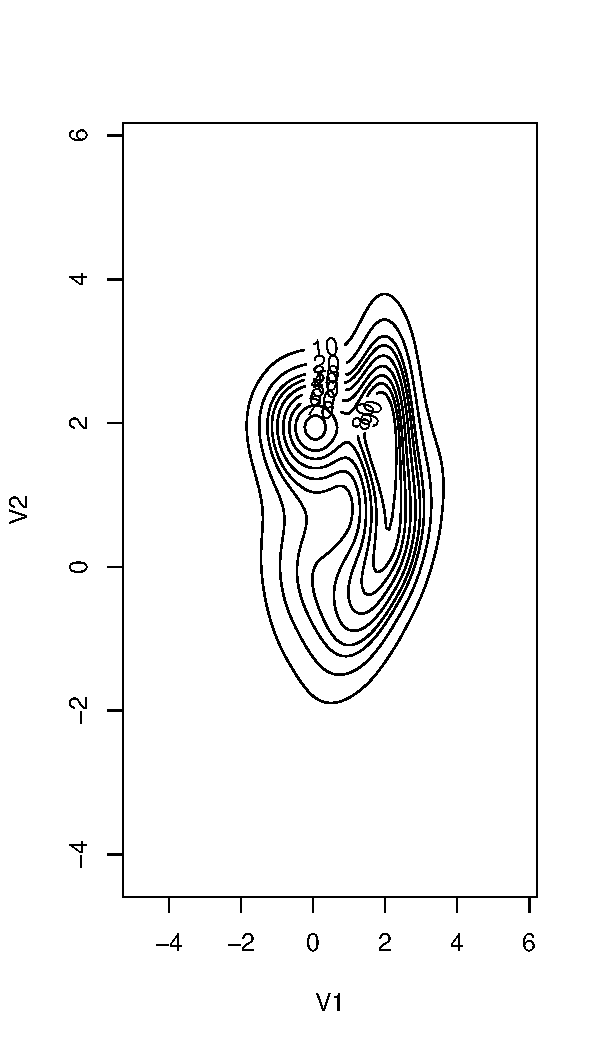
\includegraphics[height=3in]{kdeFit.pdf}
  \caption{A caption}
  \label{fig:myfig}
\end{figure}

Note the results in Fig. \ref{fig:myfig}.

\end{document}